\chapter{Molecular Dynamics}\label{ch:md}

Using the lessons learned in the previous chapter and after a reasonably successful validation of simulations (see section \ref{sec:sim_validation}), we can use the computational parameters at a lower precision and perform Molecular Dynamics simulations in VASP. The purpose of this chapter is to outline the chosen defect structures, discuss the computational details and present how defects (interstitial or otherwise) modifies the structure and dynamics of the parent structure.

\section{Computational Details}
Since Molecular Dynamics simulations require a large number of SCF cycles, it is necessary to drastically reduce the precision of our simulation. In general, the most drastic approximation comes from only running the simulation at one $k$-point ($\Gamma$). Other parameters are benchmarked by small test runs of a couple hundred steps and then evaluating the computational resources/time available. In our case we end up with the following additional reductions in precision:

\begin{itemize}
	\item Planewave cut-off at the default: \SI{400}{\eV} (\texttt{ENCUT=400})
	\item Threshold for the SCF to stop reduced to \SI{e-5}{\eV} (\texttt{EDIFF=1E-5})
	\item A faster algorithm for electronic minimization (\texttt{ALGO=F})
	\item Projection operators calculated in real space (\texttt{LREAL=A})
\end{itemize}

In addition, we need to specify the temperature and type of ensemble (see section \ref{sec:method_md}). For all simulations, we run at $T=\SI{300}{\kelvin}$ (\texttt{TEBEG=300}) within the canonical (NVT) ensemble using the algorithm of Nos\'{e} with a Nos\'{e}-mass such that the temperature fluctuates with a frequency of roughly \SI{38}{\tera\hertz} (\texttt{SMASS=1}). In order to get reasonable statistics we run with a time step $\Delta t = \SI{2}{\femto\second}$ (\texttt{POTIM=2}) for a total of 21000 (\texttt{NSW=21000}) steps, corresponding to a simulation time of \SI{42}{\pico\second}. For the analysis, we discard the first \SI{2}{\pico\second} in order to let the system equilibrate.

For the initial structures where defects have been added, we perform a geometry optimization of the supercell in order to find a structural minimum from which to start the MD simulation. Due to the reduced symmetry (compared to the phonon calculations in chapter \ref{ch:simulation}) this is a fairly expensive operation, so we perform the optimization with the same parameters as the MD simulation, except that we increase the $k$-point mesh to $4 \times 4 \times 4$ and the SCF threshold to \SI{e-6}{\eV}. Similar to our phonon calculations, we use the conjugate gradient algorithm for this minimization.

\section{Octahedral tilts}
\begin{figure}
	\centering
	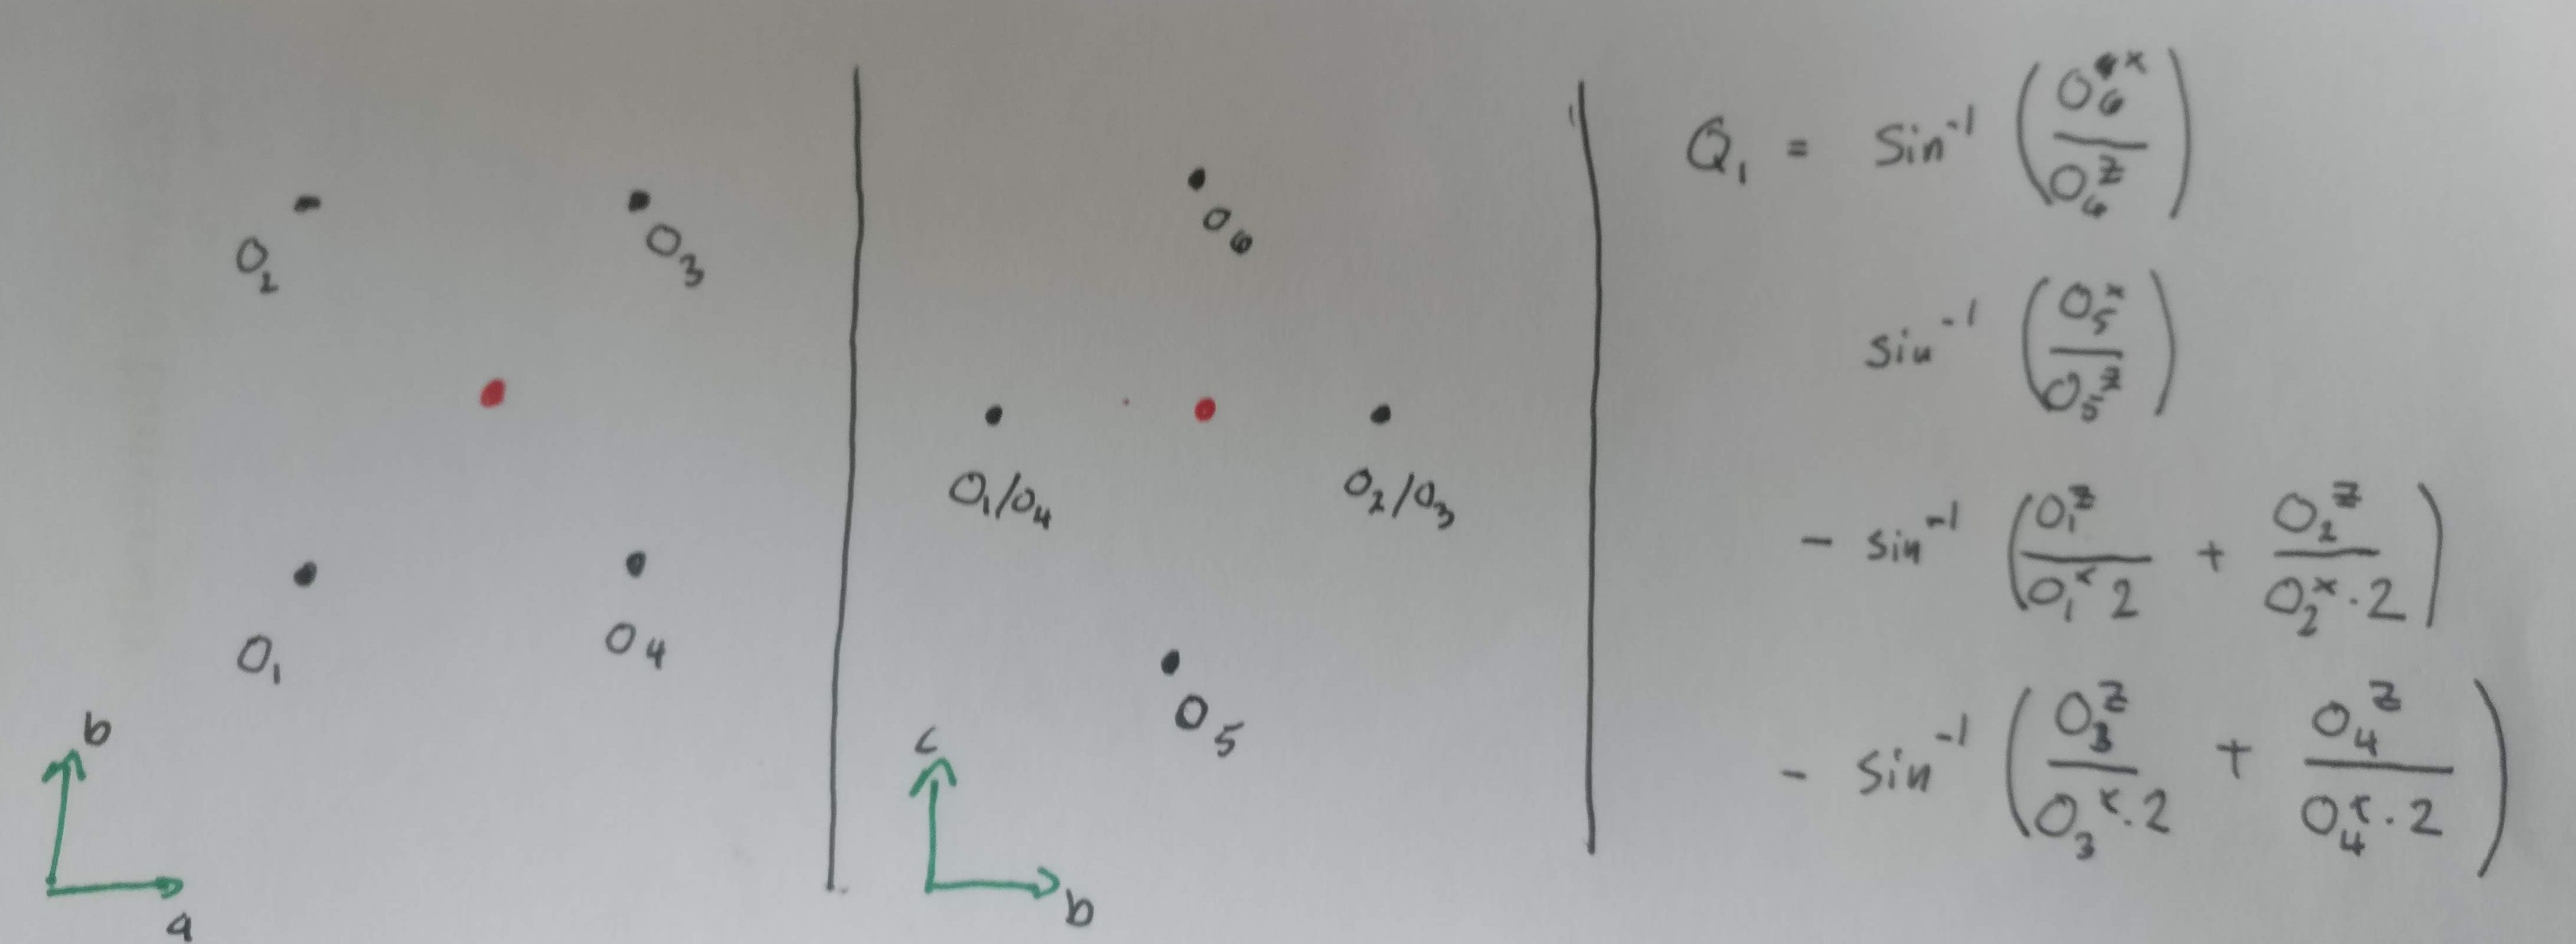
\includegraphics[width=\textwidth]{fig/md/octahedral_tilts_md.jpg}
	\caption[Finding octahedral tilts from arbitrary oxygen positions]{Finding octahedral tilts from arbitrary oxygen positions. $Q_2$ angles can be found in an analogous way by replacing $x$ with $y$ and `pairing up' O$_1$ with O$_4$ and O$_2$ with O$_3$.}
	\label{fig:md_octahedral_tilts}
\end{figure}

In order to obtain octahedral tilts from MD simulations where symmetry is P1, we are forced to define an average tilt. In fact, by writing which octahedra each oxygen atom (excluding interstitials) in our simulation belongs to, we can extract the $(Q_1,Q_2)$ tilt as seen from that oxygen. Since the tilts alternate, each tilt belongs to one of four symmetries with respect to $(Q_1,Q_2)$: (+,+), (+,-), (-,+), (-,-). In practice, we analyse the initial $t=0$ structure with the following steps for each Cu atom in the supercell:

\begin{enumerate}
	\item Record the position of the Cu atom
	\item Find apical oxygens by searching for O with a Cu-O distance less than $r = (1,1,2.7) \, \SI{}{\angstrom}$
	\item Find equatorial oxygens by searching for O with a Cu-O distance less than $r = (2.1,2.1,1) \, \SI{}{\angstrom}$
	\item Determine the $Q_1$, $Q_2$ tilt as seen from each of the 6 oxygen atoms in the list.
	\item Apply the symmetry operations.
	\item Save the 4 ($Q_1$, $Q_2$) value pairs.
\end{enumerate}

\noindent Step 4 is performed by first converting fractional coordinates to real-space coordinates and then finding angles as outlined in Figure \ref{fig:md_octahedral_tilts}. The symmetry operations in step 5 is a matrix with 8 columns corresponding to the 8 tilt values and a number of rows equal to the number of octahedra -- 16 in the case of our $2 \times 2 \times 2$ supercell. Each element of the matrix is either +1 or -1, where -1 will reverse the tilt direction and +1 will keep it as-is. The matrix can be generated by examining the output of the starting structure (which has the correct space group symmetry) and then constructing the matrix such that all tilts agree. While the same result can be archived by manually assigning the different atoms of our manageable supercell, this methodology allows the code to eventually be expanded to other systems since we can set up arbitrary local coordinate systems.

After having performed this analysis, we can apply the same operations to every time step and obtain statistics about the time-evolution of the octahedral tilts in our system. This is similar to the Positional Recurrence Maps (PRM) methodology \cite{Piovano2016} that has been used to extract dynamical information about the apical oxygen in Nd$_2$NiO$_{4+\delta}$ \cite{Perrichon2015}.

\section{Defect Structures}
Since the introduction of interstitials breaks the local crystal symmetry, we cannot perform phonon calculations using the direct method without making an excessive amount of displacement calculations. For this reason, we are forced to use ab-initio molecular dynamics, and try to come up with a reasonable model for placing the defects. In the following, we consider Sr and O-doped systems separately.

\subsection{LCO+O}
We start by considering the LCO+O System, which is simply LCO with added oxygen atoms at interstitial sites. It is generally accepted that the oxygen enters in the middle of the rock-salt layer at approximately $\left(\frac{1}{4}  \frac{1}{4} \frac{1}{4} \right)$ in fractional coordinates with respect to the orthorhombic Bmab system \cite{Rial1997}. Figure \ref{fig:oint_location} shows possible interstitial positions for the LTO (Bmab) and LTT (P4$_2$/ncm) phase, taken from a model proposed for the Nicklates \cite{Tranquada1994}. We ignore the HTT phase for molecular dynamics since the symmetry is broken and the preliminary geometry optimization would tend to tilt the octahedra similar to the LTT phase. This would make the distinguishing LTT and HTT difficult.

\begin{figure}
    \centering
    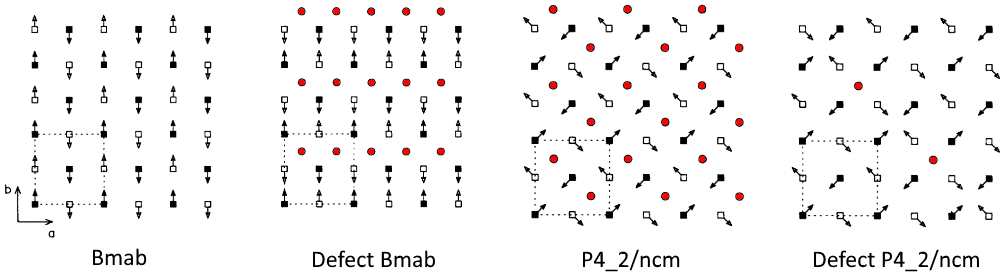
\includegraphics[width=\textwidth]{fig/md/oint.png}
    \caption[Illustration of interstitial positions]{Illustration of interstitial oxygen in-plane ($a$-$b$) location with respect to the apical oxygen displacements in the rock-salt layer. Open squares represent apical oxygens `hanging down' while closed squares represent apical oxygens `sticking up'. Interstitial oxygen are red circles. Adapted from \cite{Tranquada1994}.}
    \label{fig:oint_location}
\end{figure}

To see how the symmetry is broken, Table \ref{tab:oint_locations} shows the resulting space groups as a function of interstitial $z$-component and various defect structures in a $2 \times 2 \times 1$ supercell based on the orthorhombic crystallographic cell. 

\begin{table}
	\centering
	\caption[Oxygen interstitial phases]{Space group symmetry due to the introduction of an interstitial oxygen in various structures all described in a $2 \times 2 \times 1$ supercell of the Bmab (conventional) coordinate system. HTT, LTO and LTT are the usual phases as described in literature \cite{Hucker2012}. The structures labeled defect is (A) in the LTO case: A stacking fault where the middle layer has its tilts reversed and (B) in the LTT case: A line along [110] with reversed tilts. Both are described in \cite{Tranquada1994} and are designed in order to `make room' for the interstitial oxygen (see Figure \ref{fig:oint_location}).}
    \label{tab:oint_locations}
    \begin{tabular}{@{}lllll@{}}
\toprule
Phase                   & Space Group & $\text{O}_\text{i}^x$ & $\text{O}_\text{i}^y$ & $\text{O}_\text{i}^z$ \\ \midrule
HTT                     & I4/mmm (139)      &         &         &         \\
HTT + O$_\text{i}$      & P-42m  (111)    & 0.125   & 0.125   & 0.25    \\
HTT + O$_\text{i}$      & Cmm2 (35)       & 0.125   & 0.125   & 0.24    \\
LTO                     & Bmab (64)       &         &         &         \\
LTO + O$_\text{i}$      & P2 (3)    & 0.125   & 0.125   & 0.25    \\
LTO + O$_\text{i}$      & P2 (3)         & 0.125   & 0.125   & 0.24    \\
LTO$_\text{defect}$     & Pmna (53)       &         &         &         \\
LTO$_\text{defect}$ + O$_\text{i}$ & P2 (3)         & 0.875   & 0.375   & 0.25    \\
LTO$_\text{defect}$ + O$_\text{i}$ & P2 (3)         & 0.875   & 0.375   & 0.24    \\
LTT                     & P4$_2$/ncm (138)  &         &         &         \\
LTT + O$_\text{i}$      & P-4 (81)        & 0.375   & 0.125   & 0.25    \\
LTT + O$_\text{i}$      & P2 (3)         & 0.375   & 0.125   & 0.24    \\
LTT$_\text{defect}$               & Pmma (51)       &         &         &         \\
LTT$_\text{defect}$ + O$_\text{i}$ & Cmm2 (35)       & 0.875   & 0.375   & 0.25    \\
LTT$_\text{defect}$ + O$_\text{i}$ & Cmm2 (35)       & 0.875   & 0.375   & 0.24    \\ \bottomrule
\end{tabular}

\end{table}

We performed high-precision geometry optimizations (with symmetry turned off) on these structures (including a test of HTT) resulting in the table of energies as shown in Table \ref{tab:oint_en}. While the defect structures intuitively would make more room for oxygen interstitials, the energy cost of forming the defect is higher in the, relatively small, supercell that we use. It is worth noting, however, that they move to very similar energies during the optimization\todo{not so surprising, since they probably move towards the same structure. I need to check this more closely}.

\begin{table}[b]
	\centering
	\caption[Oxygen interstitial phases: Energy]{Oxygen interstitial phases: Energy. $E_0$ corresponds to the energy after inserting the interstitial oxygen, but before geometry optimization. $E_1$ is the total energy after optimization. Geometry optimization performed on ionic positions only. The octahedral tilts are similarly defined before and after the optimization.}
	\label{tab:oint_en}
	\begin{tabular}{@{}lllll@{}}
    \toprule
	 & $E_0$ [eV] & $E_1$ [eV] & $(Q_1, Q_2)_0$ & $(Q_1, Q_2)_1$  \\ 
	\midrule
    HTT + O$_i$                    & -827.27669             & -829.76250 & (0.00, 0.00) & (1.00, 1.00) \\
    LTO + O$_i$                    & -828.29890             & -830.39658  & (0.00, 5.79) & (1.21, 5.92) \\
    LTO$_\text{defect}$              & -823.09516             & -830.03588  & (0.00, 5.79) & (2.12, 4.48) \\
    LTT + O$_i$                    & -828.04663             & -830.08248  & (4.61, 4.61) & (3.77, 3.72) \\
	LTT$_\text{defect}$              & -826.03173             & -829.94243  & (4.61, 4.61) & (2.80, 2.70) \\ 
	\bottomrule
    \end{tabular}
\end{table}

\subsection{LSCO}

\section{Molecular Dynamics}
\[ T = \frac{1}{3 k_\text{B} (N_\text{ions}-1)} \sum_n M_n |\bm{v}_n|^2 \]
\todo[inline]{in progress... Data from LTO and LTT exists...}

\begin{figure}
	\centering
	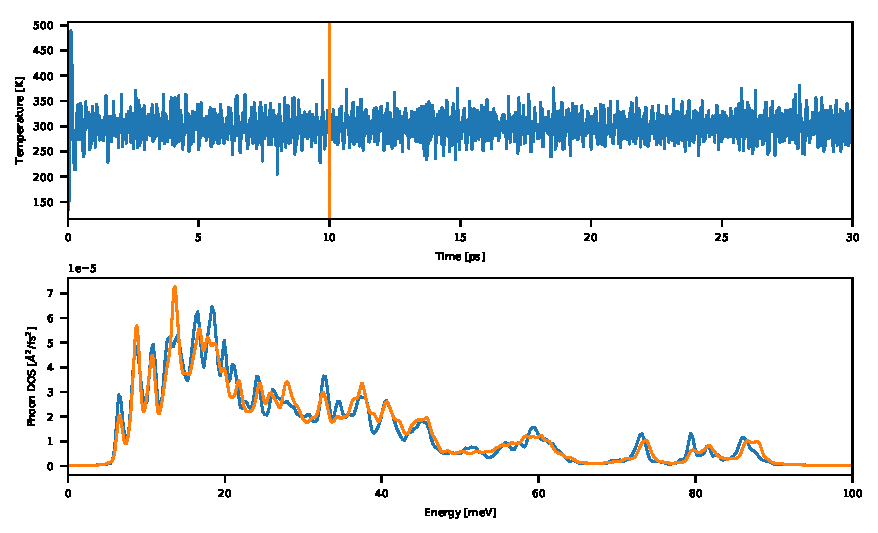
\includegraphics[width=\textwidth]{fig/md/stitch.pdf}
	\caption[stitched md runs]{sticthed md runs and comparison}
	\label{fig:stitch}
\end{figure}

\begin{figure}
	\centering
	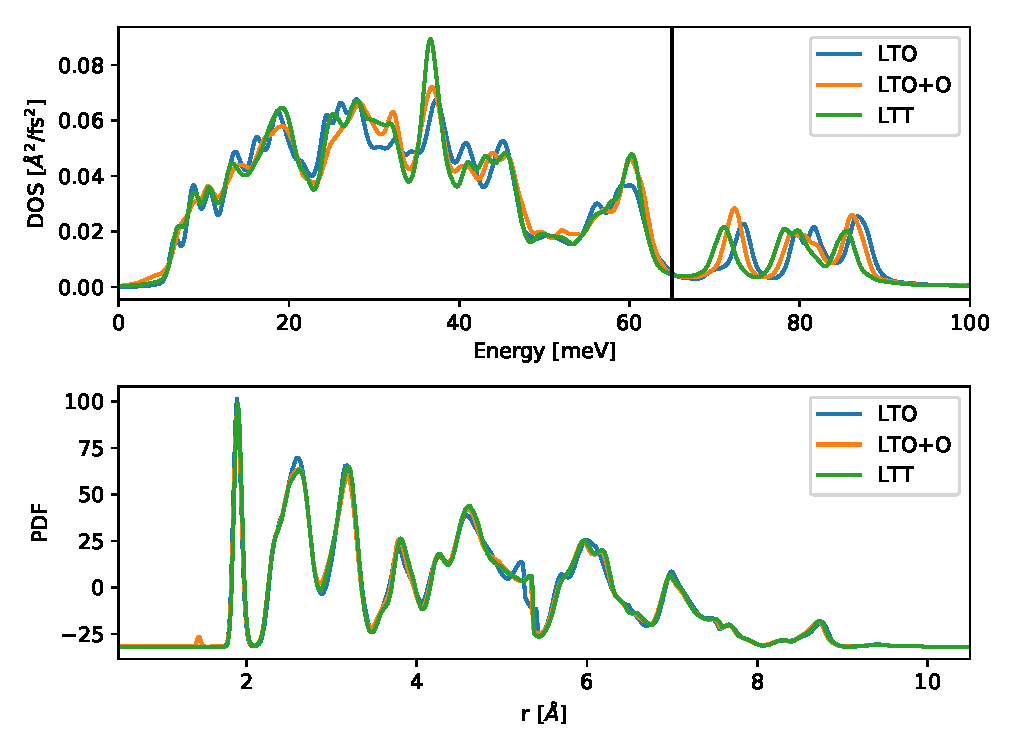
\includegraphics[width=\textwidth]{fig/md/lto_ltt_ltoo_comparison.pdf}
	\caption[MD: DOS and PDF]{MD: DOS and PDF}
	\label{fig:dos_pdf}
\end{figure}

\begin{figure}[]
	\centering
	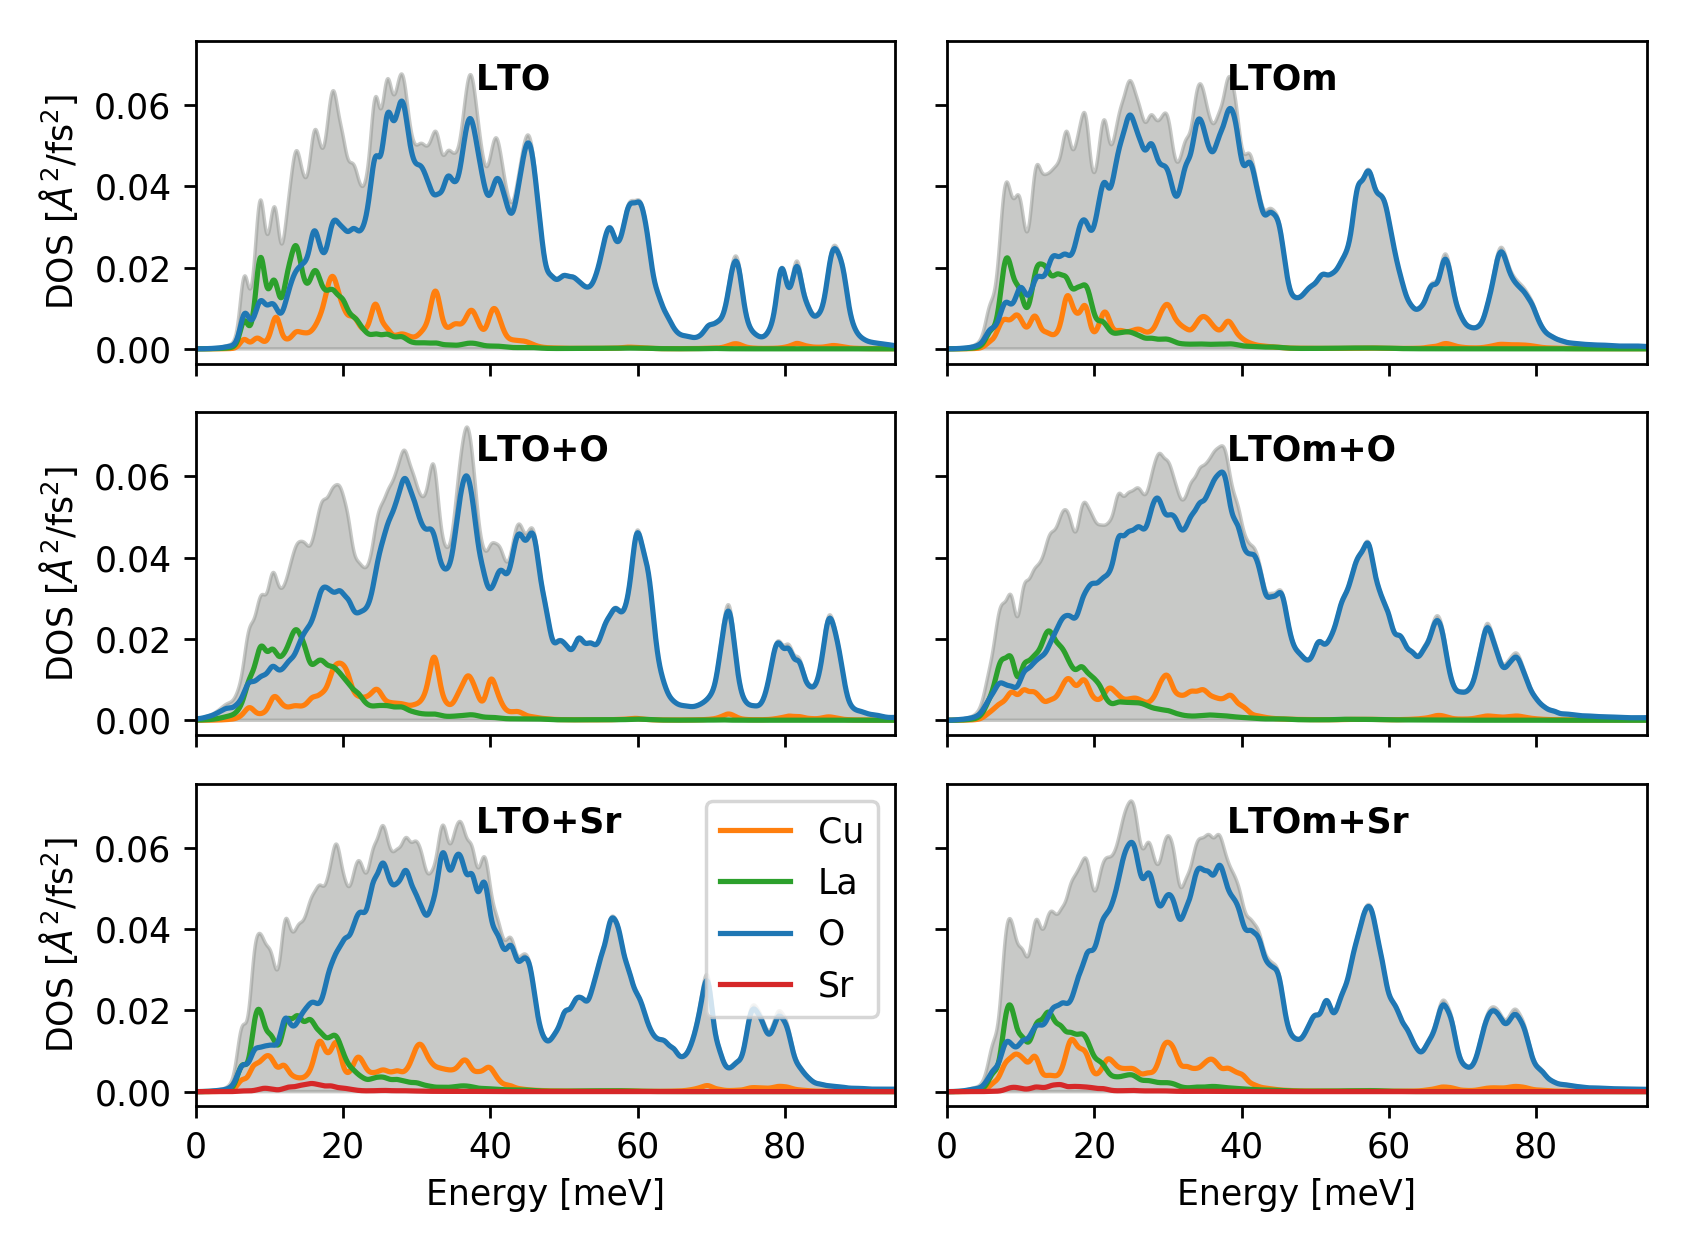
\includegraphics[width=\textwidth]{fig/md/lto_defect_comparison.png}
	\caption[LTO MD DOS: Defect comparision]{LTO MD DOS: Defect comparision}
	\label{fig:lto_md_defect_comparison}
\end{figure}

\begin{figure}
	\centering
	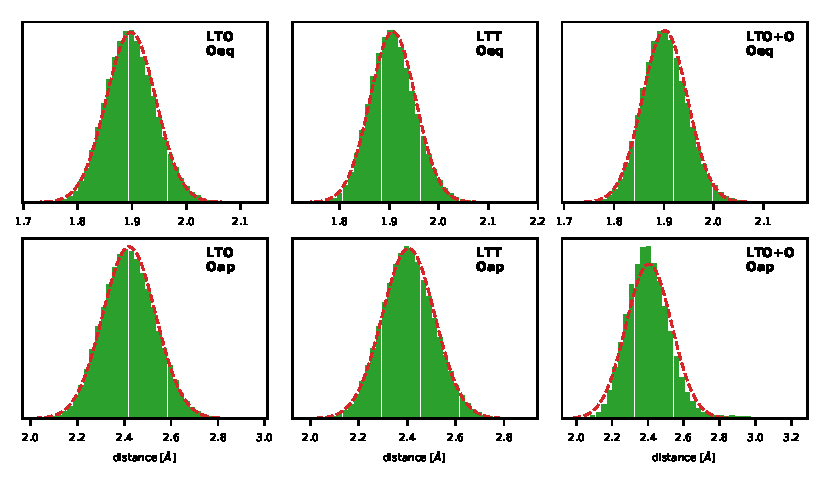
\includegraphics[width=\textwidth]{fig/md/dist_hist.pdf}
	\caption[MD: distance histograms]{MD: distance histograms}
	\label{fig:md_distances}
\end{figure}

\begin{figure}
	\centering
	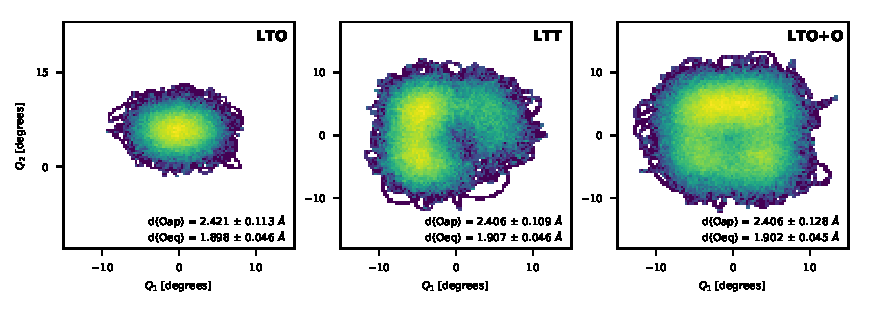
\includegraphics[width=\textwidth]{fig/md/prm_q1q2.pdf}
	\caption[MD Q1 Q2]{MD Q1 Q2}
	\label{fig:md_q1_q2}
\end{figure}

\begin{figure}
	\centering
	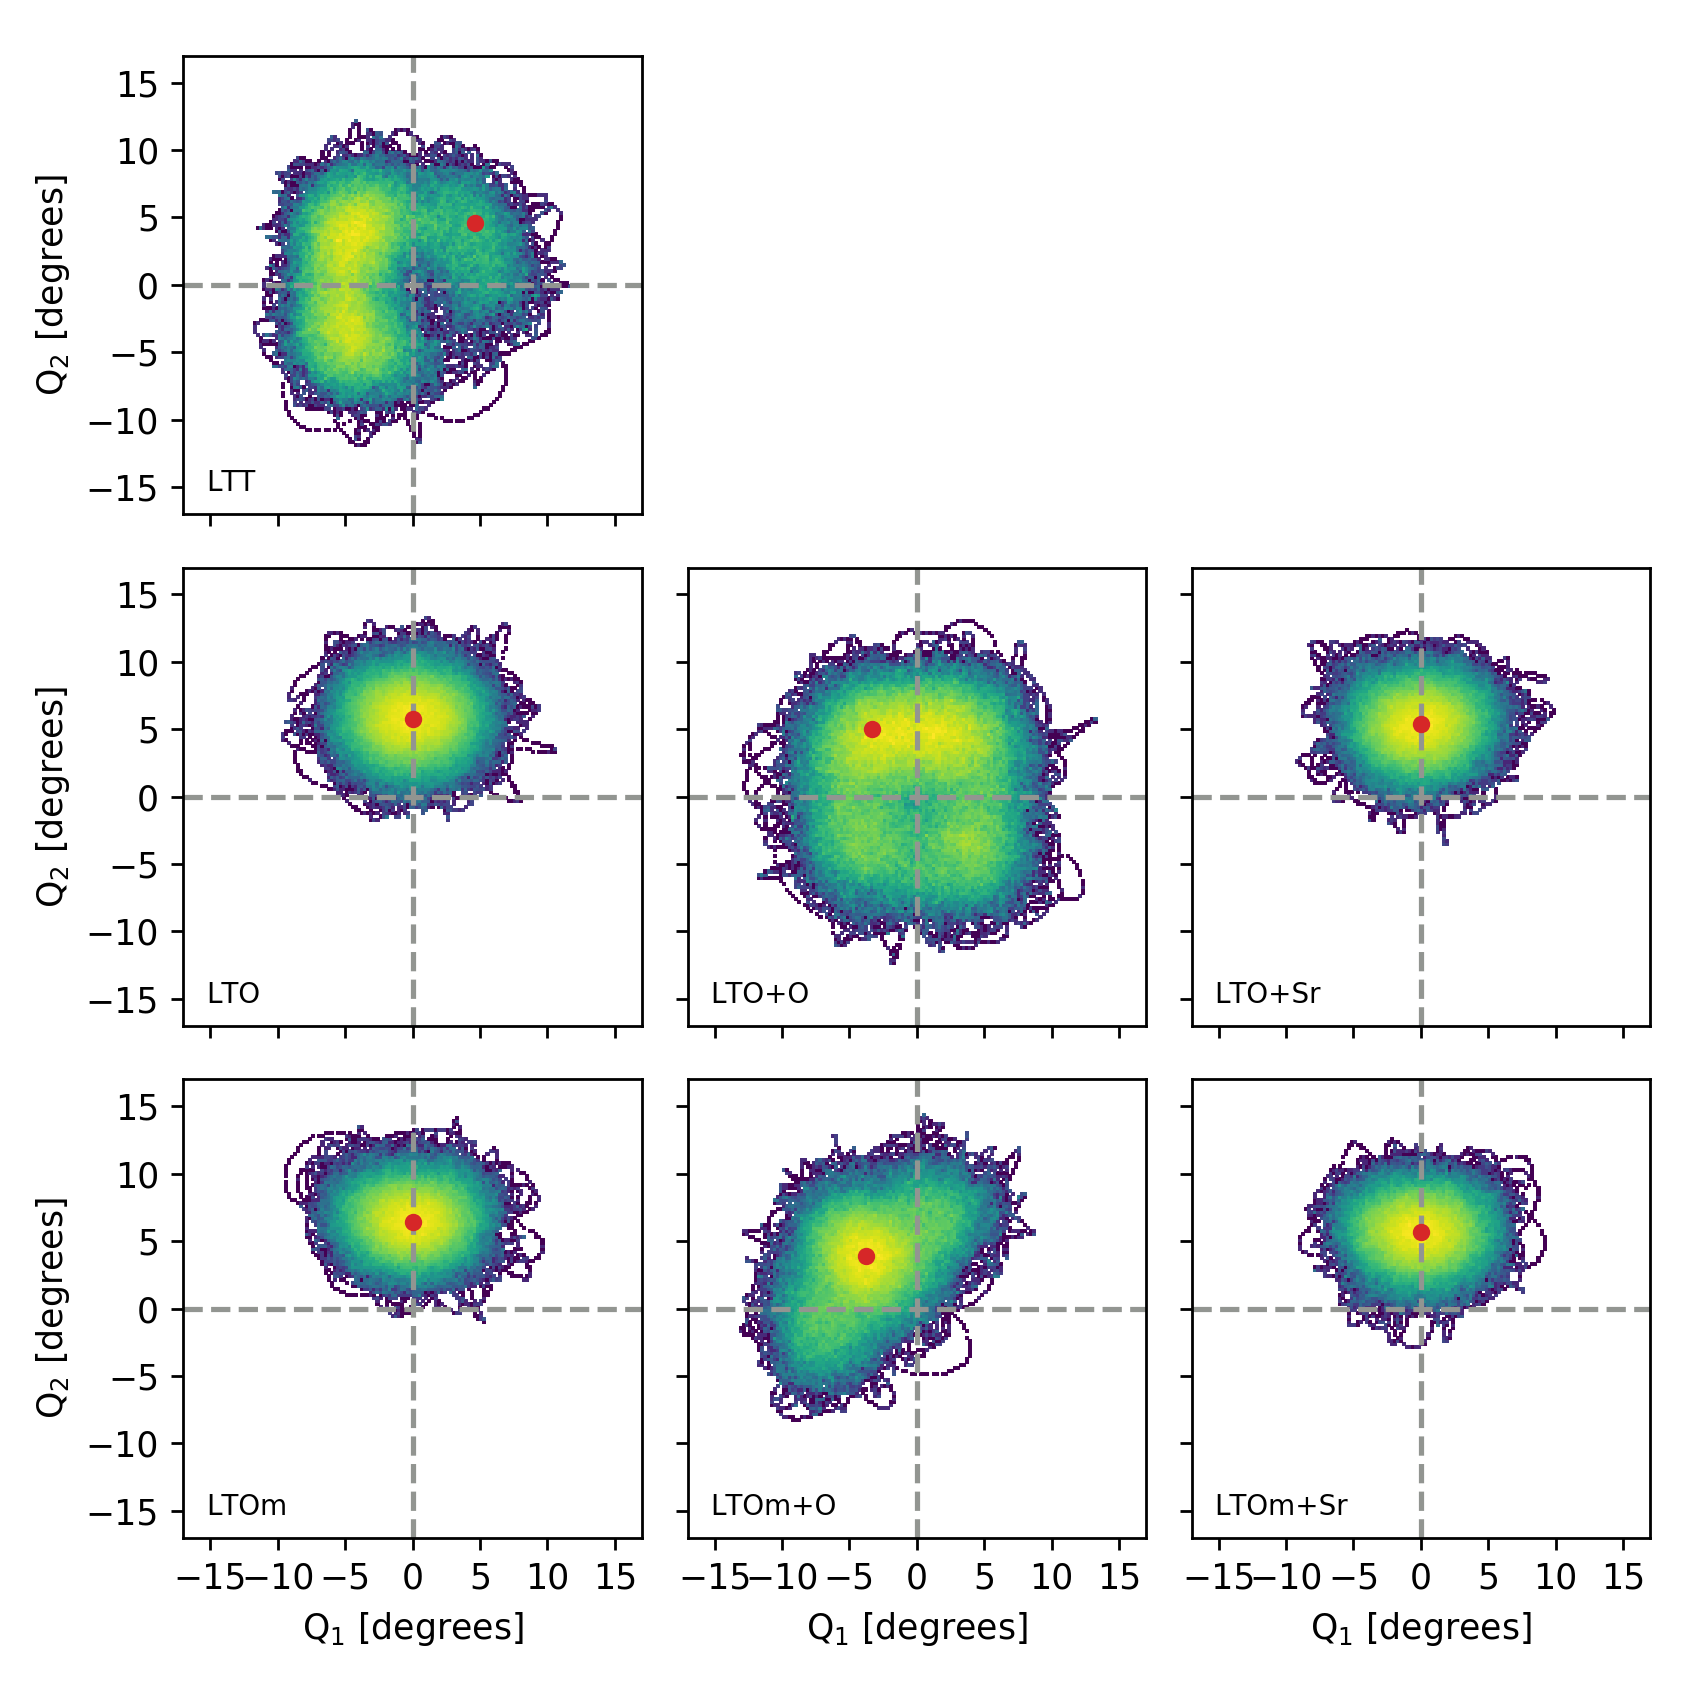
\includegraphics[width=\textwidth]{fig/md/Q1_Q2_all.png}
	\caption[MD Q1 Q2 All sims]{MD Q1 Q2 All sims}
	\label{fig:md_q1_q2_all}
\end{figure}

\begin{table}
	\centering
	\begin{tabular}{lllllll}
		\toprule
			name &   d(Oeq) & sigma(Oeq) &  R2(Oeq) &   d(Oap) & sigma(Oap) &  R2(Oap) \\
		\midrule
			 LTO &  1.89837 &  0.0454907 &  0.997277 &  2.42126 &   0.112764 &  0.998931 \\
		   LTO+O &  1.90227 &  0.0464374 &  0.997236 &  2.40559 &   0.127141 &  0.960830 \\
		  LTO+Sr &  1.89838 &  0.0507032 &  0.994707 &  2.43771 &   0.146267 &  0.999500 \\
			LTOm &  1.90897 &  0.0513818 &  0.995099 &  2.46200 &   0.140257 &  0.999679 \\
		  LTOm+O &  1.90826 &  0.0532324 &  0.993406 &  2.43961 &   0.155845 &  0.999179 \\
		 LTOm+Sr &  1.90508 &  0.0522777 &  0.994720 &  2.45116 &   0.150613 &  0.999230 \\
			 LTT &  1.90732 &  0.0460712 &  0.997086 &  2.40577 &   0.108611 &  0.999185 \\
		\bottomrule
		\end{tabular}
	\caption{MD: Cu-O Distances}
	\label{tab:md_cu_o_distances}
\end{table}

\begin{figure}
	\centering
	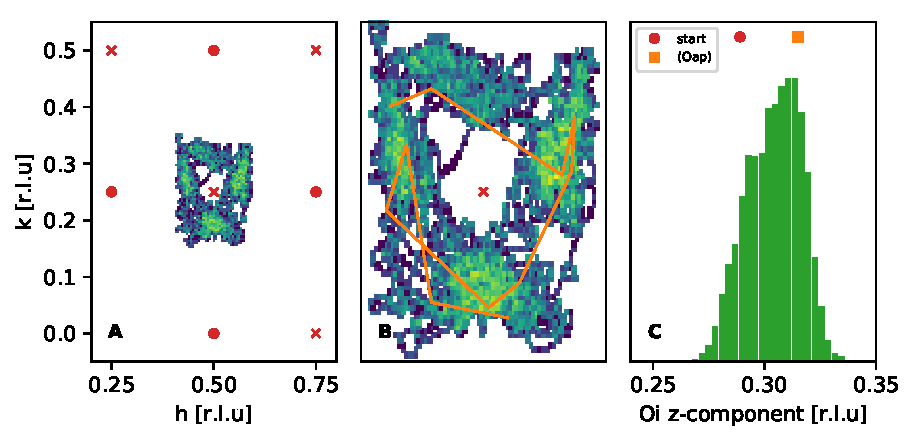
\includegraphics[width=\textwidth]{fig/md/diffusion1.pdf}
	\caption[MD Oint Diffusion Oi]{MD Oint Diffusion Oi}
	\label{fig:md_diffusion1}
\end{figure}

\begin{figure}
	\centering
	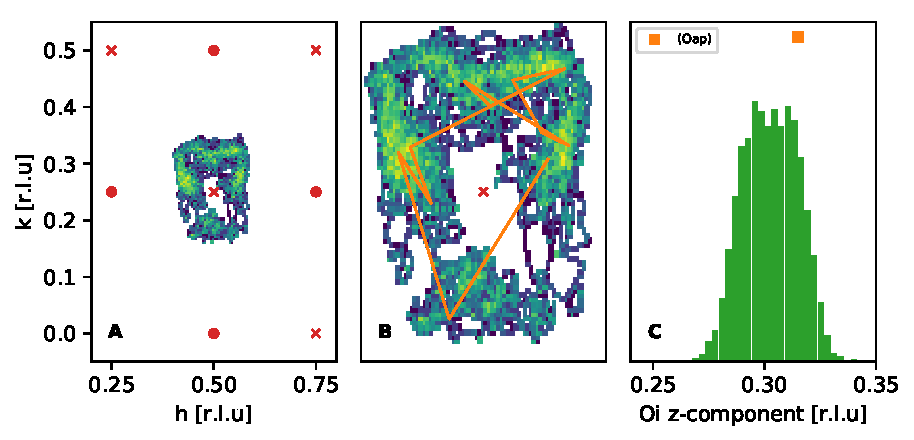
\includegraphics[width=\textwidth]{fig/md/diffusion2.pdf}
	\caption[MD Oint Diffusion Oap 1]{MD Oint Diffusion Oap 1}
	\label{fig:md_diffusion2}
\end{figure}

\begin{figure}
	\centering
	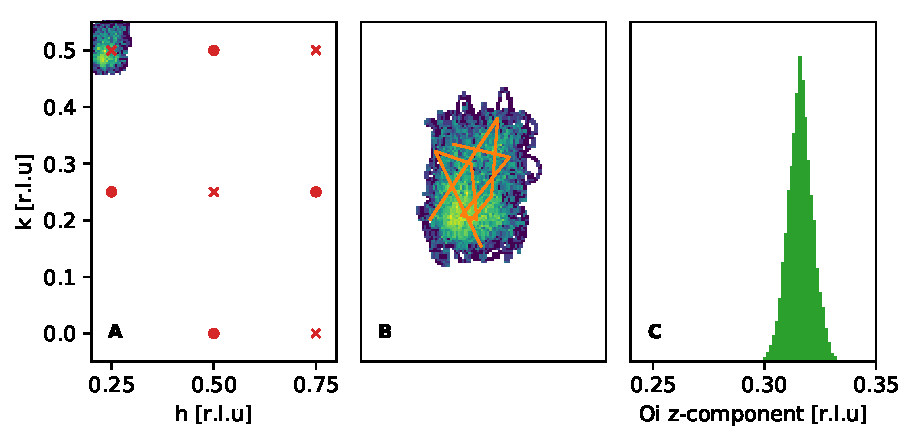
\includegraphics[width=\textwidth]{fig/md/diffusion3.pdf}
	\caption[MD Oint Diffusion Oap 2]{MD Oint Diffusion Oap 2}
	\label{fig:md_diffusion3}
\end{figure}


\begin{figure}
	\centering
	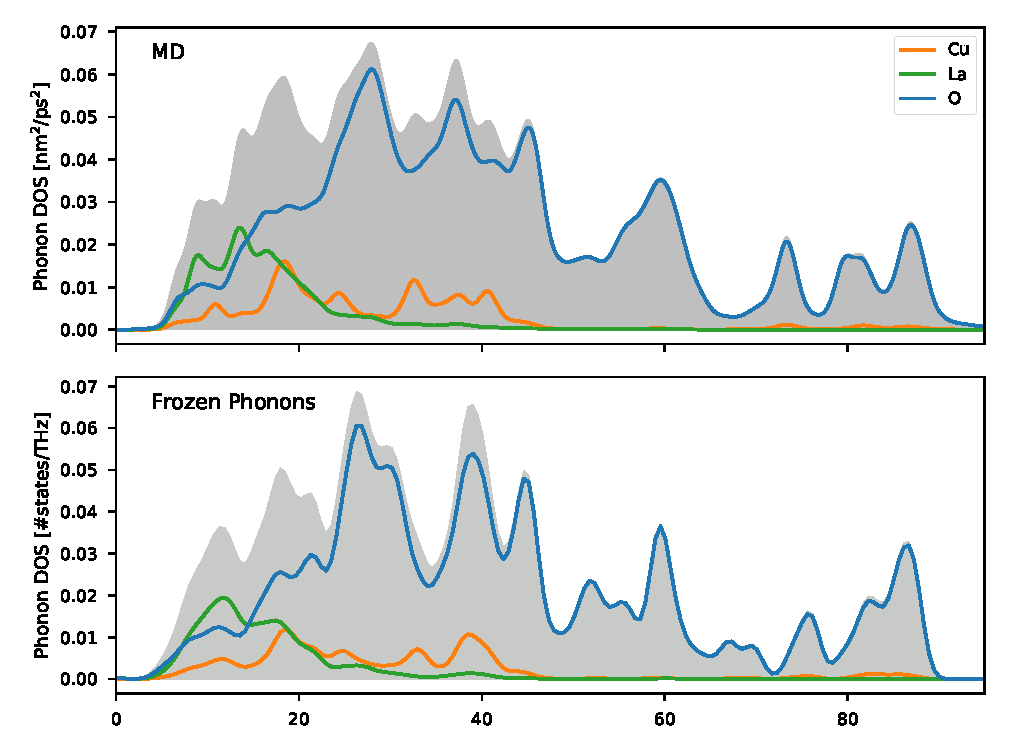
\includegraphics[width=\textwidth]{fig/md/md_phonopy_comparison.pdf}
	\caption[MD Phonopy Comparison]{MD Phonopy Comparison}
	\label{fig:md_phonopy_comparison}
\end{figure}